\documentclass[12pt, pdf, xcolor={table, dvipsnames}, paperheight=8cm,paperwidth=12cm]{beamer}
\definecolor{tugreen}{RGB}{132,184,25}
\usepackage{assets/themes/beamerthemeTUDortmund}
\usepackage{assets/themes/beamercolorthemetudortmund}

%\expandafter\def\csname ver@transparent.sty\endcsname{}
%\usepackage[edges]{forest}
%\usepackage{pgf-umlsd}
%\usepackage{dsfont}
\usepackage[utf8]{inputenc}
\usepackage[ngerman]{babel}
\usepackage[style=german,babel]{csquotes}
\usepackage{glossaries}
\makeindex
\usepackage{tabularx}
\usepackage{multirow}
\usepackage{listings}
\usepackage{amsmath}
\usepackage{graphicx}
\usepackage{calc}
\setbeamertemplate{caption}[numbered]
%\captionsetup{format=plain,indention=-3.5cm} 

%\usepackage{capt-of}
%\usepackage{pgfplots} 
%\usepackage{fontawesome}
%\usepackage{import}
%\usepackage{listings}
%\usepackage{titleref}
%\usepackage{caption}
\usepackage{tikz}
%\usepackage{../assets/tikz-uml}backend=biber
\usepackage[]{biblatex}
\addbibresource{literatur.bib}
\usetikzlibrary{backgrounds,shapes.multipart,positioning,arrows,automata,shapes.multipart,calc, fit, decorations.shapes,shadows}
\pgfdeclarelayer{myback}
\pgfsetlayers{background,main,myback}
\makeatletter
\newcommand*{\currentname}{\TR@currentTitle}
\newcommand*{\overlaynumber}{\number\beamer@slideinframe}
\makeatother
%\tikzset{
%  mylabel/.style = {font=\footnotesize, midway, fill=white, anchor=center},
%  decorate sep/.style 2 args=
%    {decorate,decoration={shape backgrounds,shape=circle,shape size=#1,shape sep=#2}},
%  invisible/.style={opacity=0, text opacity=0},
%  visible on/.style={alt={#1{}{invisible}}},
%  alt/.code args={<#1>#2#3}{%
%    \alt<#1>{\pgfkeysalso{#2}}{\pgfkeysalso{#3}} % \pgfkeysalso doesn't change the path
%  },
%  onslide/.code args={<#1>#2}{%
%  \only<#1>{\pgfkeysalso{#2}} % \pgfkeysalso doesn't change the path
%    }
%}
%\forestset{
%  step/.style={
%    /tikz/visible on={<+->},
%    edge={/tikz/visible on={<+->}},
%    for descendants={
%        /tikz/visible on={<.->},
%        edge={/tikz/visible on={<.->}}
%    }
%  },
%  highlight/.style={
%    for tree={
%      /tikz/onslide=<.>{draw=red},
%      edge+={/tikz/onslide=<.>{draw=red}}
%    }
%  }
%}
%
\author{Dennis Ochocki}
\title[]{Metamodelierte Sensordatenverarbeitung}
%\subtitle{Grafana, Prometheus und Docker}
\titlegraphic{
	
\includegraphics[width=0.35\textwidth]{./assets/themes/img/tud_logo_rgb}\hspace*{3.75cm}~%
   
\includegraphics[width=0.25\textwidth]{./assets/themes/img/fakultaet.pdf}
}
\logo{}
\institute{}
\date{\today}
\subject{}
\setbeamertemplate{navigation symbols}{}
\setbeamertemplate{frametitle}{%
    \nointerlineskip%
    \begin{beamercolorbox}[wd=\paperwidth,ht=2.6ex,dp=1.6ex]{frametitle}
        \hspace*{1ex}\insertframetitle%
    \end{beamercolorbox}%
}
\setlength{\skip\footins}{0cm}
\addtobeamertemplate{frametitle}{}{%
	\begin{tikzpicture}[remember picture,overlay]
		\node[anchor=north east,yshift=0pt] at (current page.north east) {
\includegraphics[height=0.7cm]{./assets/themes/img/fakultaet}};
	\end{tikzpicture}
}

\AtBeginSection[]{
  \begin{frame}
  \vfill
  \centering
  \begin{beamercolorbox}[sep=8pt,center,shadow=false,rounded=false]{title}
    \usebeamerfont{title}\insertsectionhead\par%
  \end{beamercolorbox}
  \vfill
  \end{frame}
}

\lstset{numbers=left, numberstyle=\tiny, stepnumber=1,firstnumber=1,
	numbersep=5pt,language=Python,
	stringstyle=\ttfamily,
	basicstyle=\footnotesize, 
	showstringspaces=false
}


\newglossaryentry{latex}
{
        name=latex,
        description={Is a mark up language specially suited for 
scientific documents}
}

\newglossaryentry{maths}
{
        name=mathematics,
        description={Mathematics is what mathematicians do}
}

\newglossaryentry{formula}
{
        name=formula,
        description={A mathematical expression}
}

\newacronym{iot}{IoT}{Internet of things}
\newacronym{pql}{PQL}{Prometheus Query Language}
\newacronym{tsdb}{TSDB}{Time Series Database}
\newacronym{promql}{PromQL}{Prometheus Query Language}
\newacronym{bzgl}{bzgl.}{bezüglich}
\newacronym{IP}{IP}{Internet Protocol}
\newacronym{IPv4}{IPv4}{Internet Protocol version 4}
\newacronym{IPv6}{IPv6}{Internet Protocol version 6}
\newacronym{ip-address}{IP-address}{Internet Protocol Address}
\newacronym{http}{HTTP}{Hyper Text Transfer Protocol}
\newacronym{ebnf}{EBNF}{Extended Backus–Naur form}
\newacronym{json}{JSON}{JavaScript Object Notation}
\newacronym{tudortmund}{TU Dortmund}{Technische Universität Dortmund}
\newacronym{ide}{IDE}{integrated development environment}
\newacronym{dsl}{DSL}{domain specific language}
\newacronym{mgl}{MGL}{meta graph language}
\newacronym{msl}{MSL}{meta style language}
\newacronym{w}{W}{Watt}
\newacronym{percent}{\%}{percent}
\newacronym{degreeC}{$^\circ$C}{degree celcius}
\newacronym{url}{URL}{Uniform Resource Locator}
\newacronym{ui}{UI}{User Interface}
\newacronym{emf}{EMF}{Eclipse Modeling Framework}
\newacronym{uml}{UML}{Unified Modeling Language}

\begin{document}
	
\maketitle

\begin{frame}{Übersicht}
	\tableofcontents
\end{frame}

\section{Motivation}
\begin{frame}{Motivation}
	Smart Home ist immer präsenter und dank \gls{iot} einfacher den je. Immer mehr Geräte, sog. \enquote{Smart Devices}, kommen auf den Markt, die in solche Systeme integriert werden können. 
	
	\begin{block}{Eigenschaften von Smart Home:}
		\begin{itemize}
			\item Viele verschiedene Smart Devices in einem Netzwerk
			\item Jedes Gerät ist Sensor und/oder Akteur
			\item Dient der Qualitätssteigerung der vernetzten Örtlichkeit
			\item Eine zentrale Logikkomponente verarbeitet die Informationen
		\end{itemize}
	\end{block}
\end{frame}

\begin{frame}{Motivation}
	Sei gegeben ein Raum mit einem Thermometer und einem Thermostat.
	
	\vspace{1em}
	Das Thermometer (Sensor) misst regelmäßig die Raumtemperatur, eine zentrale Logik verarbeitet diese Werte und kann passend dazu das Thermostat (Akteur) steuern.
	
	\vspace{1em}
	Solche und andere Automatismen dienen der Verbesserung situationsabhängiger Qualitäten.
	
	\begin{tikzpicture}[]	
	\node[] at (0, 0) {};
	\node[] at (\paperwidth - 9cm, 0) {
\includegraphics[height=1cm]{assets/images/lightbulb-solid}};
	\node[] at (\paperwidth - 7cm, 0) {
\includegraphics[height=1cm]{assets/images/bolt-solid}};
	\node[] at (\paperwidth - 5cm, 0) {
\includegraphics[height=1cm]{assets/images/wind-solid}};
	\node[] at (\paperwidth - 3cm, 0) {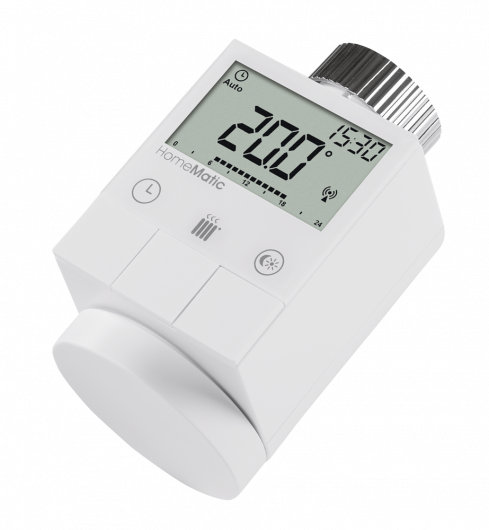
\includegraphics[height=2cm]{assets/images/thermostat}};
	\end{tikzpicture}
\end{frame}

\begin{frame}{Motivation}
	Meist sind die Anwendungsfälle trivial und einfach zu realisieren, damit schöpft man aber nicht alles an Funktionalität aus, was möglich wäre.
	\begin{block}{Was sind die Schwierigkeiten?}
		\begin{itemize}
			\item Bei vielen Smart Devices ist es schwer den Überblick zu behalten
			\item Assoziationen von Geräte-IP zur physikalischer Position muss gemerkt werden
			\item Muss nicht auf eine Wohnung begrenz sein, mehrere Örtlichkeiten, Häuser oder Städte möglich
			\item Geeignete/übersichtliche Visualisierung finden
		\end{itemize}
	\end{block}
thermostat.png
\end{frame}


\section{Grundlagen}

\begin{frame}{Senoren und Akteure}
	Sensoren und Akteure sind die atomaren Bestandteile eines solchen Netzwerkes.
	
	\vspace{1em}
	Sensoren liefern Metriken und Aktuere können auf das Umfeld einwirken um damit auf die erfassten Werte zu reagieren.
	\begin{block}{Beispiel: Sensor}
		\vspace{0.5em}
		\begin{tabularx}{\linewidth}{lX}Thermometer: & Erfasst Temperatur, stellt Werte zur  Verfügung
		\end{tabularx}
	\end{block}
	\begin{block}{Beispiel: Akteur}
	\vspace{0.5em}
	\begin{tabularx}{\linewidth}{lX}Thermostat: &Steuert Heizung, hat Einfluss auf die Temperatur
	\end{tabularx}
	\end{block}
Ein Gerät kann ein Sensor und/oder ein Akteur sein.
\end{frame}

\begin{frame}{Metrik}
	Eine Metrik ist ein Merkmal welches vom Sensor erfasst wird.
	
	\vspace{1em}
	Sei gegeben ein Smart Device, hier: Wetterstation.
	
	\vspace{1em}
	\noindent
	\begin{columns}
		\begin{column}{.5\linewidth}
			\begin{block}{Beispiel: Metriken}
				\vspace{.5em}
				\begin{tabularx}{\linewidth}{lX}
					Luftfeuchtigkeit & Wert in \%\\
					Luftdruck & Wert in hPa\\
					Temperatur & Wert in °C\\
				\end{tabularx}
			\end{block}
		\end{column}%
		\begin{column}{.45\linewidth}
			\begin{figure}[h]
				\centering
				\centering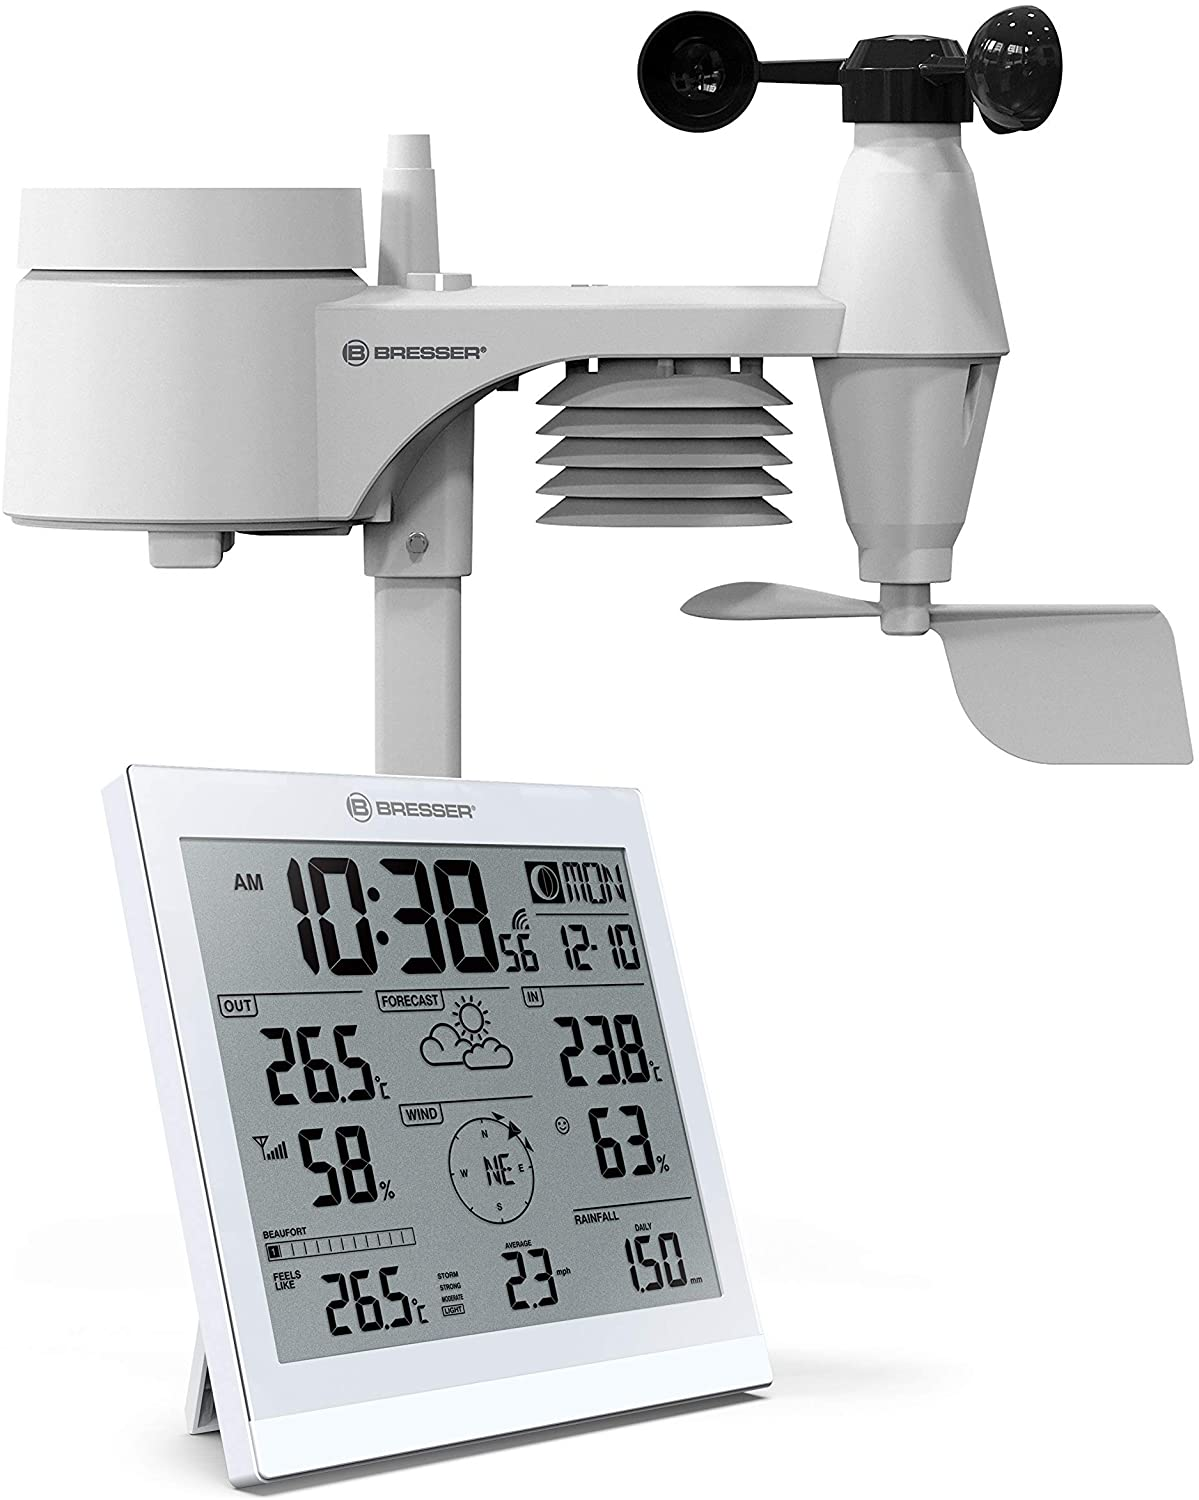
\includegraphics[width=0.5\textwidth]{assets/images/wetterstation.jpg}
				\caption{Wetterstation\footnotemark[1]}
				\label{fig:mesh1}
			\end{figure}
		\end{column}%
	\end{columns}
\footnotetext[1]{www.bresser.de}
\end{frame}


\begin{frame}{Architektur}
	\centering
	\begin{tikzpicture}[n/.style={draw,thick,circle,inner sep=0pt,minimum width=1cm}]
	\setbeamercovered{invisible}
	\uncover<1->{%
		\node [n, label=Luftfeuchtigkeit] (M1) {$M_1$};
		\node [n, below = 1cm of M1, label=Temperatur] (M2) {$M_2$};
		\node [n, below = 1cm of M2, label=Luftdruck] (M3) {$M_3$};
	}
	\uncover<2->{%
		\node [n, right = 2cm of M1, label=Wetterstation] (S1) {$S_1$};
		\draw [->] (M1) -- (S1) (M2) -| ($ (M2) !.5! (S1) $) |- (S1) (M3) -| ($ (M3) !.5! (S1) $) |- (S1);
	}
	\uncover<3->{%
		\node [n, below = 1cm of S1] (S2) {$S_2$};
		\node [n, below = 1cm of S2] (S3) {$S_3$};
	}
	\uncover<4->{%
		\node [n, right = 2cm of S2, label=Prometheus] (P) {$P$};
		\draw [->] (S1) -- (P);
		\draw [->](S2) -- (P);
		\draw [->] (S3) -- (P);
	}
	\uncover<5->{%
		\node [n, right = 2cm of P, label=Grafana] (G) {$G$};
		\draw [->] (P) -- (G);
	}
	\end{tikzpicture}
\end{frame}

\begin{frame}{Prometheus}
	Prometheus ist eine Systemüberwachungs- und Benachrichtigungssoftware
	
	\vspace{1em}
	Es greift selbstdefinierte Schnittstellen der Sensoren ab um darüber Metriken zu lesen und in der internen \gls{tsdb} abzuspeichern.
	
	\vspace{1em}
	Über die \gls{pql} kann man auf diese Daten zugreifen.
	
	\begin{tikzpicture}[remember picture,overlay]
	\draw (current page.north east) -- +(0,-1.1) coordinate (b);
	\node[anchor=north east,yshift=0pt] at (b) {
\includegraphics[height=2cm]{./assets/images/200px-Prometheus_software_logo.svg}};
	\end{tikzpicture}
\end{frame}

\begin{frame}[fragile]{Prometheus - Sensor}
	Sensoren können in der Konfigurationsdatei angebunden werden und liefern nach folgendem Standard folgende Ausgabe:
	
	\vspace{1em}
	\url{GET} \url{http://sensor:3001/metrics}
		\begin{onlyenv}<1>
			\begin{lstlisting}[firstnumber=1, label=glabels,xleftmargin=10pt, frame=single, gobble=12, tabsize=4, mathescape]
			# HELP luftfeuchtigkeit in %
			# TYPE luftfeuchtigkeit gauge
			luftfeuchtigkeit 86
			
			# HELP luftdruck in hPa
			# TYPE luftdruck gauge
			luftdruck 1005
			
			# HELP temperatur in ${^\circ}$C
			# TYPE temperatur gauge
			temperatur 23.3
			\end{lstlisting}
		\end{onlyenv}
		\begin{onlyenv}<2>
			\begin{lstlisting}[firstnumber=1, label=glabels,xleftmargin=10pt, frame=single, gobble=12, tabsize=4, mathescape]
			# HELP luftfeuchtigkeit in %
			# TYPE luftfeuchtigkeit gauge
			luftfeuchtigkeit 84
			
			# HELP luftdruck in hPa
			# TYPE luftdruck gauge
			luftdruck 1003
			
			# HELP temperatur in ${^\circ}$C
			# TYPE temperatur gauge
			temperatur 22.9
			\end{lstlisting}
		\end{onlyenv}
\end{frame}

\begin{frame}{Grafana}
	Grafana dient dem Darstellen und der Analyse\\
	 jener Daten, die durch z.B. Prometheus gewonnenen Daten.
	
	\vspace{1em}
	Alternativ zu Prometheus können auch andere Datenquellen wie z.B. JSON, Cassandra, MySQL, \dots angebunden werden.
	
	\vspace{1em}
	Die Daten können in Tabellen, Grafen, Balkendiagrammen und anderen Diagrammarten dargestellt werden.
	
	\begin{tikzpicture}[remember picture,overlay]
	\draw (current page.north east) -- +(0,-1.1) coordinate (b);
	\node[anchor=north east,yshift=0pt] at (b) {
\includegraphics[height=2cm]{./assets/images/1200px-Grafana_logo.svg}};
	\end{tikzpicture}
\end{frame}

\begin{frame}{Grafana}
	\begin{tikzpicture}
	\node[at=(current page.center)] {%
		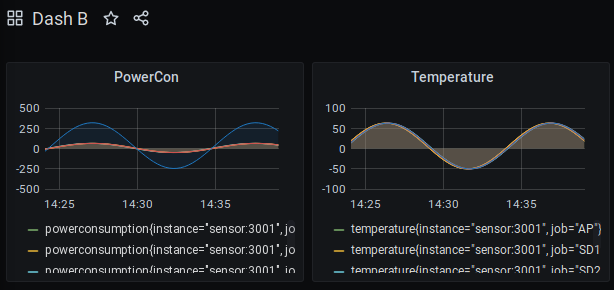
\includegraphics[keepaspectratio,%
		width=\paperwidth-1cm,%
		height={\paperheight-1cm}]{./assets/images/grafana-image}%
	};
	\end{tikzpicture}
\end{frame}

\section{MetricArchitect}
\begin{frame}{MetricArchitect}
	Um all diese Technologien und Probleme zusammenzufassen, soll ein Tool für die Generierung der Konfiguration verantwortlich sein.
	\begin{block}{Vision}
		\begin{itemize}
			\item Ein zentraler Punkt um alle Einstellungen zu setzen
			\item Best-Of-Breed Lösungen aus der Wirtschaft sorgen für die Zukunftsfähigkeit des Projektes
			\item Kann als Verwaltung und Übersicht komplexer Netzwerke genutzt werden
			\item Durch abstrakte Modellierung entstehen wiederverwendbare Komponenten
		\end{itemize}
	\end{block}
\end{frame}


\begin{frame}{MetricArchitect}
	Das komplexe System kann in vier Ebenen unterteilt werden, welche zusammen  alle Informationen beinhalten, um alle erforderlichen Dateien zu generieren
	
	\begin{block}{Abstraktionsebenen:}
		\begin{itemize}
			\item Sensoren
			\item Physikalische Platzierung
			\item Logische Aufbereitung
			\item Projektspezifikationen
		\end{itemize}
	\end{block}
\end{frame}




\begin{frame}{MetricArchitect}
	Diese Art von Projekt, in der alles beschrieben ist, kann bei Bedarf angepasst werden und mit dem geplanten Docker-Deployment auch direkt wieder ausgerollt werden.
	
	\vspace{1em}
	Da alle Informationen an einem Ort sind, ist eine Wartung auch einfach möglich.
	
	
	\begin{center}
		\begin{tikzpicture}
		\node[] at (0, 0) {
\includegraphics[height=2cm]{assets/images/docker}};
		\node[] at (\paperwidth - 8cm, 0) {
\includegraphics[height=2cm]{assets/images/k8s}};
		\end{tikzpicture}
	\end{center}
	
\end{frame}

\begin{frame}{MetricArchitect}
	\LARGE\centering{$<Live Demo>$}
\end{frame}


\begin{frame}{Zeitplan}
\begin{tikzpicture}

\node [rounded corners=3mm, minimum width=\linewidth, minimum height=7cm, fill=gray!10] (wrapper) {};

\draw[draw=gray!50] ([xshift=-{(\linewidth-1cm)*0.27},yshift=-2mm]wrapper.north) -- ([xshift=-{(\linewidth-1cm)*0.27},yshift=2mm]wrapper.south);
\draw[draw=gray!50] ([xshift={(\linewidth-1cm)*0.27},yshift=-2mm]wrapper.north) -- ([xshift={(\linewidth-1cm)*0.27},yshift=2mm]wrapper.south);
\draw[draw=gray!50] ([xshift={(\linewidth-1cm)*0.0},yshift=-2mm]wrapper.north) -- ([xshift={(\linewidth-1cm)*0.0},yshift=2mm]wrapper.south);

\node at ([xshift=-(\linewidth-1cm)*.405]$ (wrapper.north) !.1! (wrapper.south)$) [rounded corners=3mm, minimum width=(\linewidth-1cm)*.19, minimum height=.7cm, fill=gray!20] {Mon. 1};
\node at ([xshift=-(\linewidth-1cm)*.135]$ (wrapper.north) !.1! (wrapper.south)$) [rounded corners=3mm, minimum width=(\linewidth-1cm)*.19, minimum height=.7cm, fill=gray!20] {Mon. 2};
\node at ([xshift=(\linewidth-1cm)*.135]$ (wrapper.north) !.1! (wrapper.south)$) [rounded corners=3mm, minimum width=(\linewidth-1cm)*.19, minimum height=.7cm, fill=gray!20] {Mon. 3};
\node at ([xshift=(\linewidth-1cm)*.405]$ (wrapper.north) !.1! (wrapper.south)$) [rounded corners=3mm, minimum width=(\linewidth-1cm)*.19, minimum height=.7cm, fill=gray!20] {Mon. 4};

\node at ([xshift=-(\linewidth-1cm)*.405]$ (wrapper.north) !.3! (wrapper.south)$) [rounded corners=3mm, minimum width=(\linewidth-1cm)*0.19, minimum height=.7cm, fill=gray!20] {Impl.};

\node at ([xshift=-{(\linewidth-1cm)*.27}]$ (wrapper.north) !.5! (wrapper.south)$) [rounded corners=3mm, minimum width={(\linewidth-1cm)*0.46}, minimum height=.7cm, fill=gray!20] {Recherche};

\node at ([xshift=-{(\linewidth-1cm)*.135}]$ (wrapper.north) !.7! (wrapper.south)$) [rounded corners=3mm, minimum width={(\linewidth-1cm)*0.73}, minimum height=.7cm, fill=gray!20] {Thesis schreiben};

\node at ([xshift={(\linewidth-1cm)*0.405}]$ (wrapper.north) !.9! (wrapper.south)$) [rounded corners=3mm, minimum width={(\linewidth-1cm)*0.19}, minimum height=.7cm, fill=gray!20] {Korr.};


\end{tikzpicture}
\end{frame}

\begin{frame}{Zusammenfassung}
	Es handelt sich bei MetricArchitect um die Idee einer Zusammenfassung verschiedenster Lösungen für verschiedene Probleme um große Projekte zur realisieren.
	 
	\vspace{1em}
	Aufgebaut ist das ganze auf Best-Of-Breed Lösungen um selbst bei Wegfall von MetricArchitect eine Wartung zu ermöglichen.
	\begin{center}
		\begin{tikzpicture}
		\node[] at (0, 0) {
\includegraphics[height=2cm]{assets/images/200px-Prometheus_software_logo.svg}};
		\node[] at (\paperwidth - 8cm, 0) {
\includegraphics[height=2cm]{assets/images/1200px-Grafana_logo.svg}};
		\end{tikzpicture}
	\end{center}
\end{frame}

\section{Ausblick}
\begin{frame}{Ausblick}
	Features:
	\begin{itemize}
		\item Funktionsverschachtelung $sum(abs(x))$
		\item Mehrere Standorte ordentlich abbildbar
		\item Definierung der Kachelgrößen/Position in Grafana
		\item Vollständige Abbildung der \gls{pql}
		\item Verifizierung beim Modelieren
		\item \dots
	\end{itemize}
\end{frame}

%\begin{frame}[plain,allowframebreaks]{Verwandte Arbeiten}
	%\nocite{*}
	%\printbibliography[heading=none, keyword={related}]
%\end{frame}

%\begin{frame}[plain,allowframebreaks]{Mögliche Literatur}
	%\printbibliography[heading=none, keyword={possible}]
%\end{frame}

%\begin{frame}[plain,allowframebreaks]{Abbildungsverzeichnis}
	%\printbibliography[heading=none, keyword={image}]
%\end{frame}
\end{document}